\documentclass[11pt,final,hidelinks]{article}
\usepackage{lmodern}
\usepackage[T1]{fontenc}
\usepackage[english]{babel}
\usepackage[utf8]{inputenc}
\usepackage[activate={true,nocompatibility},final,tracking=true,kerning=true,
    spacing=true,factor=1100,stretch=10,shrink=10]{microtype}
\microtypecontext{spacing=nonfrench}
\usepackage[margin=1in]{geometry}
\usepackage{graphicx}
\graphicspath{{img/}}
\usepackage{caption}
\usepackage{subcaption}
\usepackage{booktabs}
\usepackage{array}
\usepackage{mathtools}
\usepackage{enumitem}
\usepackage{commath}
\usepackage{appendix}
\renewcommand\appendixtocname{Appendices}
\usepackage{amsmath}
\usepackage{amsthm}
\usepackage{amssymb}
\usepackage{pgfplots}
\usepackage{tikz}
\usepackage{tikzscale}
\usepackage[square,numbers]{natbib}
\bibliographystyle{plain}
\usepackage{siunitx}
\numberwithin{equation}{section}
\usepackage[hypertexnames=false]{hyperref}
\usepackage{cleveref}

\pgfplotsset{compat=newest}

\usepackage[fancy,section]{alex}

\hypersetup{
    pdftitle={Entropy and space complexity of random approximate sets},
    pdfauthor={Alexander Towell},
    pdfsubject={computer science},
    pdfkeywords={
        Shannon entropy,
        space complexity,
        approximate set,
        Bloom filter,
        information-theoretic lower bound,
        Bernoulli set},
    colorlinks=true,
    linkcolor=magenta,
    citecolor=green,
    filecolor=blue,
    urlcolor=green
}

\title
{
    Entropy and space complexity of random approximate sets
}
\author
{
    Alexander Towell\\
    \texttt{atowell@siue.edu}
}
\date{2026}

\begin{document}
\maketitle
\begin{abstract}
We derive the joint entropy of the false positive and false negative error counts in the Bernoulli set model---a compositionally closed framework for random approximate sets with independent, element-wise errors.
The joint entropy decomposes additively via element independence and admits a closed-form asymptotic expansion based on the binomial entropy approximation.
We then establish the information-theoretic space lower bound for positive approximate sets over countably infinite universes, restating and proving the classical result of Carter, Floyd, Gill, Markowsky, and Wegman in the notation of the Bernoulli framework.
The Bloom filter achieves $\ln 2 \approx 69\%$ of the optimal density.
The general case---approximate sets with both false positives and false negatives ($0 < \tprate < 1$)---remains an open problem.
\end{abstract}

\microtypesetup{protrusion=false}
\tableofcontents
\microtypesetup{protrusion=true}

%%%%%%%%%%%%%%%%%%%%%%%%%%%%%%%%%
% Introduction
%%%%%%%%%%%%%%%%%%%%%%%%%%%%%%%%%
\section{Introduction}
\label{sec:intro_ent}

The Bernoulli set model~\cite{bernoulliSets} provides a compositional framework
for random approximate sets---data structures whose membership queries may err
with known false positive and false negative rates.
A natural information-theoretic question is: how much uncertainty do these
errors carry?

\paragraph{Motivation.}
The joint entropy of error counts quantifies the inherent unpredictability of a
Bernoulli set realization.
This entropy has direct implications for coding: any lossless representation of
the error pattern requires at least this many bits on average.
The space complexity question---how many bits are needed to implement an
approximate set---connects the abstract Bernoulli model to the concrete cost of
probabilistic data structures.

\paragraph{Contribution.}
We make two contributions.
First, we derive the joint entropy of the false positive and false negative
counts (\cref{thm:joint_entropy_fp_fn}), showing that it decomposes additively
by element independence and admits the closed-form asymptotic expansion
\begin{equation}
    \log_2(2\pi e)
    + \frac{1}{2}\log_2\!\bigl(
        (u-m) \cdot m \cdot \fprate(1-\fprate) \cdot \fnrate(1-\fnrate)
      \bigr)
    + \mathcal{O}\!\left(\frac{u}{m(u-m)}\right).
\end{equation}
We extend this to the case where the number of positives is itself uncertain
(\cref{sec:entropy:pos_neg}).
Second, we restate and prove the classical space lower bound of Carter et
al.~\cite{carterExact} for positive approximate sets
(\cref{pst:approx_l_b}): any implementation over a countably infinite universe
requires at least $-\log_2 \fprate$ bits per element.
We compare this to the Bloom filter's $-(1/\ln 2)\log_2\fprate$ bits per
element and note that the general case $0 < \tprate < 1$ remains open
(\cref{rem:general_lower_bound}).

\paragraph{Related work.}
Shannon~\cite{shannonBSC} introduced the entropy of binary channels; Cover and
Thomas~\cite{coverThomas} provide the binomial entropy expansion we use.
Carter et al.~\cite{carterExact} established the space lower bound.
Bloom~\cite{bf} introduced the eponymous filter.
The Bernoulli set model and its compositional algebra are developed in a
companion paper~\cite{bernoulliSets}.

\paragraph{Organization.}
\Cref{sec:prelim_ent} restates the Bernoulli axioms.
\Cref{sec:entropy} derives the joint entropy.
\Cref{sec:space_comp} establishes the space complexity lower bound.
\Cref{sec:conclusion_ent} concludes with open problems.

%%%%%%%%%%%%%%%%%%%%%%%%%%%%%%%%%
% Preliminaries
%%%%%%%%%%%%%%%%%%%%%%%%%%%%%%%%%
\section{Preliminaries}
\label{sec:prelim_ent}

We restate the elements of the Bernoulli set model~\cite{bernoulliSets} used in
this paper.

\begin{axiom}[Element-wise independence]
\label{asm:element_indep}
For all distinct $x, y \in U$, the error events at $x$ and $y$ are mutually independent:
\begin{equation}
P(\mathbf{1}_{\tilde{A}}(x) \neq \mathbf{1}_{A}(x) \mid \mathbf{1}_{\tilde{A}}(y) \neq \mathbf{1}_{A}(y)) =
	P(\mathbf{1}_{\tilde{A}}(x) \neq \mathbf{1}_{A}(x)).
\end{equation}
More generally, the family $\{\mathbf{1}_{\tilde{A}}(x) : x \in U\}$ is mutually independent given the objective set $A$ and the error rates.
Furthermore, within each partition block $B_i$, the error indicators $\{\mathbf{1}_{\tilde{A}}(x) : x \in B_i\}$ are identically distributed.
\end{axiom}

\begin{axiom}[Conditional independence of block error rates]
\label{asm:fpr_fnr_r_indep}
Given the objective set $R$, the random error rates $\alpha_1, \ldots, \alpha_n$ for the respective partition blocks $B_1, \ldots, B_n$ are mutually independent.
\end{axiom}

From these axioms, the false positive count
$\FP_m \sim \bindist(u-m, \fprate)$ and the false negative count
$\FN_m \sim \bindist(m, \fnrate)$ are conditionally independent given $m$
positives in a universe of $u$ elements~\cite{bernoulliSets}.

%%%%%%%%%%%%%%%%%%%%%%%%%%%%%%%%%
% Entropy of approximate sets
%%%%%%%%%%%%%%%%%%%%%%%%%%%%%%%%%%%
\section{Entropy of approximate sets}
\label{sec:entropy}
The Bernoulli set model assigns binomial distributions to the number of false
positives and false negatives.
A natural question is how much \emph{uncertainty} these error counts carry,
as measured by Shannon entropy~\cite{shannonBSC}.
In this section, we derive the joint entropy of the false positive and false
negative counts and extend the analysis to the case in which the number of
positives is itself uncertain.

\begin{theorem}[Joint entropy of false positives and false negatives]
\label{thm:joint_entropy_fp_fn}
Given $m$ positives in a universe of $u$ elements, the joint entropy of the
uncertain number of false positives and false negatives in a Bernoulli set with
expected false positive rate $\fprate$ and expected false negative rate $\fnrate$
is
\begin{equation}
\label{eq:joint_entropy}
    \Entropy{\FP_m, \FN_m}
    = \log_2(2\pi e)
    + \frac{1}{2}\log_2\!\bigl(
        (u - m) \cdot m \cdot \fprate(1-\fprate) \cdot \fnrate(1-\fnrate)
      \bigr)
    + \mathcal{O}\!\left(\frac{u}{m(u-m)}\right),
\end{equation}
where the asymptotic term holds as $u \to \infty$ with $m/u$ bounded away
from $0$ and $1$ (so that both $m$ and $u - m$ grow with $u$).
\end{theorem}
\begin{proof}
By \cref{asm:element_indep}, the random error counts $\FP_m$ and $\FN_m$
are conditionally independent given $m$ positives (they are functions of
indicators on disjoint element sets: negatives and positives respectively).
Therefore the joint entropy decomposes additively:
\begin{equation}
    \Entropy{\FP_m, \FN_m} = \Entropy{\FP_m} + \Entropy{\FN_m}.
\end{equation}
The random variable $\FP_m$ is binomially distributed,
$\FP_m \sim \operatorname{Bin}(u - m,\, \fprate)$.
The entropy of a binomial distribution $\operatorname{Bin}(n, p)$ admits the
well-known asymptotic expansion~\cite{coverThomas}
\begin{equation}
\label{eq:binomial_entropy_asymp}
    H = \frac{1}{2}\log_2\!\bigl(2\pi e \cdot n \cdot p(1-p)\bigr)
      + \mathcal{O}(1/n).
\end{equation}
Applying \cref{eq:binomial_entropy_asymp} to $\FP_m$ and $\FN_m$ respectively
yields
\begin{align}
    \Entropy{\FP_m}
    &= \frac{1}{2}\log_2(2\pi e)
     + \frac{1}{2}\log_2\!\bigl((u-m)\,\fprate(1-\fprate)\bigr)
     + \mathcal{O}\!\left(\frac{1}{u-m}\right), \\
    \Entropy{\FN_m}
    &= \frac{1}{2}\log_2(2\pi e)
     + \frac{1}{2}\log_2\!\bigl(m\,\fnrate(1-\fnrate)\bigr)
     + \mathcal{O}\!\left(\frac{1}{m}\right).
\end{align}
Summing these expressions and combining the logarithms gives
\begin{equation}
    \Entropy{\FP_m, \FN_m}
    = \log_2(2\pi e)
    + \frac{1}{2}\log_2\!\bigl(
        (u-m)\, m\, \fprate(1-\fprate)\, \fnrate(1-\fnrate)
      \bigr)
    + \mathcal{O}\!\left(\frac{u}{m(u-m)}\right),
\end{equation}
where the error term follows from
$\mathcal{O}(1/(u-m)) + \mathcal{O}(1/m)
 = \mathcal{O}\!\bigl(u / (m(u-m))\bigr)$.
\end{proof}

\subsection{Positives and negatives}
\label{sec:entropy:pos_neg}
When the number of positives is itself uncertain, modeled by the random
variable $\POS$ with probability mass function $\Fun{p}_{\POS}(p \Given u)$,
the joint distribution of positives, false positives, and false negatives
factorizes as
\begin{equation}
\label{eq:joint_pos_fp_fn}
    \Fun{p}(p, f_p, f_n \Given u, \fprate, \fnrate)
    = \Fun{p}_{\POS}(p \Given u)
      \;\Fun{p}_{\FP}(f_p \Given p, u, \fprate)
      \;\Fun{p}_{\FN}(f_n \Given p, u, \fnrate).
\end{equation}
By \cref{asm:element_indep}, $\FP$ and $\FN$ are conditionally independent
given $\POS$, so the joint entropy decomposes as
\begin{equation}
\label{eq:joint_entropy_pos}
    \Entropy{\POS, \FP, \FN}
    = \Entropy{\POS}
    + \sum_{p=0}^{u} \Fun{p}_{\POS}(p \Given u)\, \Entropy{\FP \Given p}
    + \sum_{p=0}^{u} \Fun{p}_{\POS}(p \Given u)\, \Entropy{\FN \Given p}.
\end{equation}
The last two sums are the conditional entropies $\Entropy{\FP \Given \POS}$
and $\Entropy{\FN \Given \POS}$, each weighted by the distribution of
positives.

\begin{example}
The \emph{expected} number of false positives, marginalizing over $\POS$, is
\begin{align}
    \Expect{\FP}
    &= \sum_{p=0}^{u} \Fun{p}_{\POS}(p \Given u)\, \Expect{\FP_p}
     = \sum_{p=0}^{u} \Fun{p}_{\POS}(p \Given u)\, (u - p)\,\fprate \notag \\
    &= \fprate \bigl(u - \Expect{\POS}\bigr)
     = \fprate \cdot \Expect{\NEG},
\end{align}
confirming that the marginal expected false positive count depends only on the
expected number of negatives and the false positive rate $\fprate$.
\end{example}

%%%%%%%%%%%%%%%%%%%%%%%%%%%%%%%%%
% Space complexity
%%%%%%%%%%%%%%%%%%%%%%%%%%%%%%%%%
\section{Space complexity}
\label{sec:space_comp}

If the finite cardinality of a universe is $u$ and the set is \emph{dense} (and the approximation is also dense, i.e., the false negative rate is relatively
small), then
\begin{equation}
    \mathcal{O}(u) \; \si{bits}
\end{equation}
are needed to code the set, which is independent of $\p$, the false positive rate, and the false negative rate.

The lower-bound on the \emph{expected} space complexity of a data structure that models the \emph{positive random approximate set} where the elements are over a \emph{countably infinite} universe is a classical result due to Carter, Floyd, Gill, Markowsky, and Wegman~\cite{carterExact}.
We restate it here in the notation of the present paper and include a proof for completeness.
\begin{proposition}[{\cite{carterExact}}]
\label{pst:approx_l_b}
The \emph{information-theoretic lower-bound} of a data structure that implements the countably infinite \emph{positive random approximate set} abstract data type has an \emph{expected} bit length given by
\begin{equation}
    -\log_2 \fprate \; \si{bits \per element},
\end{equation}
where $\fprate > 0$ is the false positive rate.
\end{proposition}
\begin{proof}
It suffices to prove the bound for deterministic encodings; the extension to randomized data structures follows from Yao's minimax principle.

Consider a finite subset of the universe with $n$ elements, from which an
objective set $S$ of size $\p$ is drawn.
A deterministic encoding using $B$ bits maps each input set $S$ to a state
$r = f(S)$ from at most $2^B$ distinct states.
Each state $r$ determines a \emph{positive response set}
$Q(r) = \{x : \text{query}(x,r) = 1\}$.
Since the data structure has no false negatives ($\tprate = 1$), we have
$S \subseteq Q(r)$ for the state $r = f(S)$ encoding $S$.
The false positive rate constraint requires that at most an $\fprate$-fraction of the $n - \p$ negatives belong to $Q(f(S))$ for every input set $S$, so
$|Q(f(S))| \leq \p + \fprate(n - \p)$ for all $S$.
In particular, $|Q(r)| \leq \p + \fprate(n - \p)$ for every state $r$ in the image of $f$.

By the pigeonhole principle, some state $r^*$ must encode at least
$\binom{n}{\p} / 2^B$ distinct input sets.
Every such set is a subset of $Q(r^*)$ of size $\p$, so
\begin{equation}
\binom{n}{\p} / 2^B
    \leq \binom{|Q(r^*)|}{\p}
    \leq \binom{\p + \fprate(n - \p)}{\p}.
\end{equation}
Taking logarithms and rearranging:
\begin{equation}
B \geq \log_2 \binom{n}{\p} - \log_2 \binom{\p + \fprate(n - \p)}{\p}.
\end{equation}
For fixed $\p$ as $n \to \infty$, $\binom{n}{\p} \sim n^\p / \p!$ and
$\binom{\p + \fprate n}{\p} \sim (\fprate n)^\p / \p!$, so
\begin{equation}
B \geq \log_2 \frac{n^\p}{(\fprate n)^\p}
    = \p \log_2 \frac{1}{\fprate}
    = -\p \log_2 \fprate,
\end{equation}
giving $-\log_2 \fprate$ bits per element.
\end{proof}
\begin{remark}
\label{rem:general_lower_bound}
The general case $0 < \tprate < 1$ remains open.
When false negatives occur, $S \not\subseteq Q(r)$ and the pigeonhole step
above fails: valid input sets are no longer constrained to be subsets of the
positive response set.
The heuristic scaling $-\tprate \log_2 \fprate$ (retaining $\p \tprate$
elements on average, each requiring $-\log_2 \fprate$ bits) is plausible
but is not a valid information-theoretic lower bound, since the encoding
problem changes qualitatively when elements are randomly dropped.
\end{remark}

A well-known implementation of countably infinite \emph{positive approximate set} is the Bloom filter~\cite{bf} which has an expected space complexity given
by
\begin{equation}
    -\frac{1}{\ln 2} \log_2 \fprate \; \si{bits \per element},
\end{equation}
thus the absolute efficiency of the Bloom filter is $\ln 2 \approx 0.69$.
A practical implementation of the \emph{positive random approximate set} is given by the \emph{Perfect Hash Filter}~\cite{phf}, which compares favorably to the Bloom filter in many circumstances.\footnote{The \emph{Singular Hash Set}~\cite{shs} is an example of a data structure that obtains optimality using \emph{brute-force} search, so it is not practical for even relatively small objective sets. However, its primary purpose is analytic tractability.}

\begin{figure}[ht]
\centering
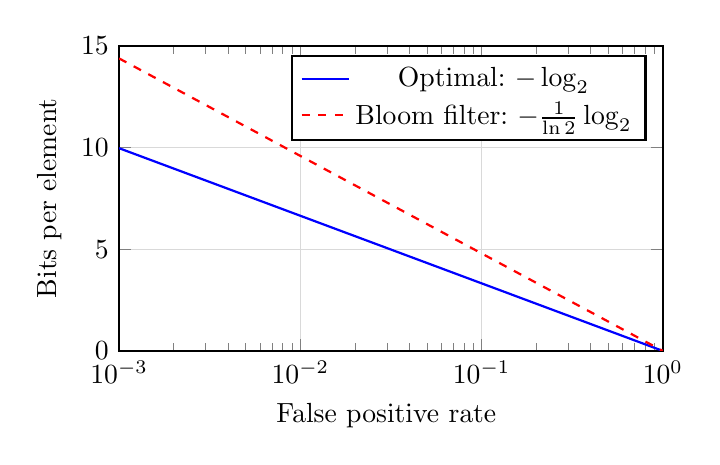
\begin{tikzpicture}
\begin{axis}[
	width=0.7\textwidth,
	height=0.45\textwidth,
	xlabel={False positive rate $\fprate$},
	ylabel={Bits per element},
	xmin=0.001, xmax=1,
	ymin=0, ymax=15,
	xmode=log,
	legend pos=north east,
	ymajorgrids, xmajorgrids,
	major grid style={gray!30},
	thick,
	samples=200,
	domain=0.001:1,
]
\addplot[blue, solid] {-ln(x)/ln(2)};
\addlegendentry{Optimal: $-\log_2 \fprate$}
\addplot[red, dashed] {-ln(x)/ln(2)/ln(2)};
\addlegendentry{Bloom filter: $-\frac{1}{\ln 2}\log_2 \fprate$}
\end{axis}
\end{tikzpicture}
\caption{Space complexity of positive approximate sets as a function of
the false positive rate $\fprate$.
The solid curve is the information-theoretic lower bound
$-\log_2 \fprate$ bits per element (\cref{pst:approx_l_b}).
The dashed curve is the Bloom filter cost
$-(1/\ln 2)\log_2 \fprate$; the gap reflects the Bloom filter's
$\ln 2 \approx 69\%$ efficiency.}
\label{fig:space_lower_bound}
\end{figure}

\documentclass[ ../main.tex]{subfiles}
\providecommand{\mainx}{..}
\begin{document}
\section{Conclusion}
\label{sec:conclusion}

We have defined the \emph{Bernoulli map}, a probabilistic function $\APFun{f}[\fprate][\fnrate] \colon \Set{X} \to \Maybe{\Set{Y}}$ that approximates an objective map $\Fun{f} \colon \Set{X} \to \Set{Y}$ with per-element errors modeled as independent Bernoulli trials. This generalizes the Bernoulli set model~\cite{aset} from indicator functions $\Set{X} \to \BitSet$ to arbitrary codomains.

The central theoretical result is the composition theorem (\cref{sec:composition}), which shows that the composition of independent Bernoulli maps is itself a Bernoulli map and derives the resulting error rates in closed form. The false negative rate of a composition satisfies $\fnrate_{g \circ f} = 1 - (1-\fnrate_1)(1-\fnrate_2)$, while the false positive rate depends on the interaction between the false positive value distribution of the first map and the domain of the second.

We also showed that the model specializes to several important cases: the Bernoulli set (indicator functions), the binary symmetric and asymmetric channels (Bernoulli Booleans), and approximate constants (maps from the unit type).

The entropy map (\cref{sec:entropy-maps}) provides a space-optimal realization of the first-order Bernoulli map model, and the singular hash map (\cref{sec:shm}) is a concrete construction that achieves the information-theoretic lower bound of $-\log_2 \fprate + \mu$ bits per element asymptotically. Trapdoor entropy maps extend this to privacy-preserving settings relevant to encrypted search~\cite{songWagnerPerrig2000,curtmola2006}.

\paragraph{Two perspectives, one theorem.}
The function-space viewpoint developed here takes a \emph{denotational} approach: every Bernoulli approximation is a latent function $\Fun{f'} \colon \Set{X} \to \Set{Y}$ approximated per-input, and the Kronecker factorization of the joint confusion matrix is the structural theorem.
A companion paper on random approximate algebraic types takes the \emph{constructive} counterpart: approximate types are built from Bool using sum, product, and exponential type constructors.
Product types preserve the Kronecker factorization (parameters grow additively); sum types break it (tag errors couple the components); and the exponential type $\Set{A} \to \Set{B}$ is precisely the function space studied here.
The two perspectives converge at the exponential type, arriving at the same factorization theorem from opposite directions.
Bernoulli sets are the special case $\Set{Y} = \BitSet$; the optional type $\Set{A} + \Unit$ (a sum) recovers Bernoulli set membership as a type-theoretic construction.

\paragraph{Future directions.}
Monte Carlo validation of the composition error bounds, particularly the dependence on the parameter $\rho$ governing false-positive overlap, remains to be developed.
The relational algebra operators (join, project, select) produce non-trivial error propagation when applied to approximate relations (sets of tuples), and merit further investigation.

\end{document}


\bibliography{references}

\end{document}
